\begin{figure}[h]
    \centering
    \begin{subfigure}[b]{0.48\columnwidth}
        \centering
        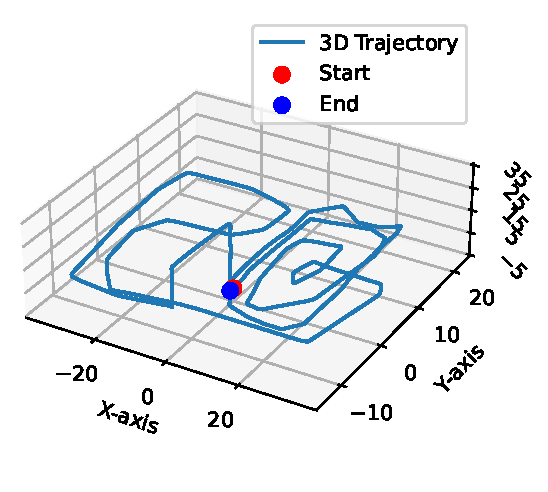
\includegraphics[width=\textwidth]{tex/ch5_airio/figs/pegasus_trajs/pegasus_0_train_test_sorted.pdf}
        \caption{TRAIN\_1: Distance 516.2$\si{\meter}$, Duration 254.7~\unit{\second}, Peak 4.8, Avg. 2.0~\unit{\metre\per\second}.}
        \label{fig:airio:sub_train1}
    \end{subfigure}
    \hfill
    \begin{subfigure}[b]{0.48\columnwidth}
        \centering
        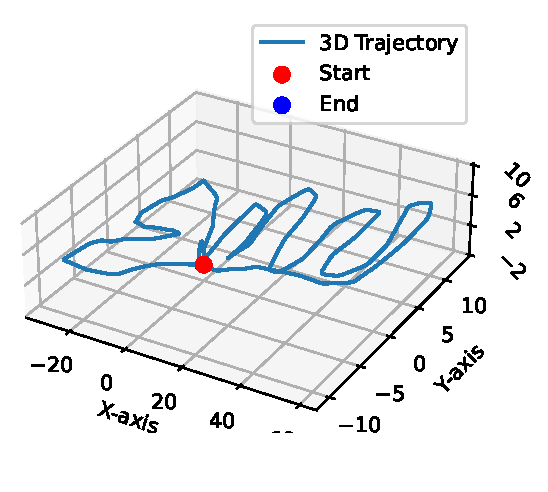
\includegraphics[width=\textwidth]{tex/ch5_airio/figs/pegasus_trajs/pegasus_1_train_test_sorted.pdf}
        \caption{TRAIN\_2: Distance 329.0$\si{\meter}$, Duration 165.8~\unit{\second}, Peak 4.3, Avg. 2.0~\unit{\metre\per\second}.}
        \label{fig:airio:sub_train2}
    \end{subfigure}

    \vspace{1em}
    \begin{subfigure}[b]{0.48\columnwidth}
        \centering
        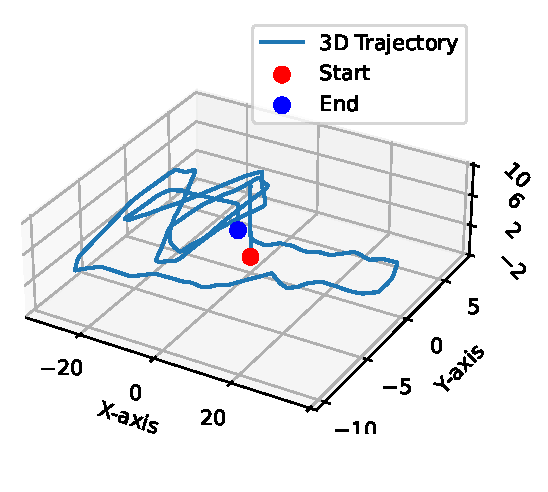
\includegraphics[width=\textwidth]{tex/ch5_airio/figs/pegasus_trajs/pegasus_2_train_test_sorted.pdf}
        \caption{TRAIN\_3: Distance 263.5$\si{\meter}$, Duration 355.5~\unit{\second}, Peak 4.6, Avg. 0.7~\unit{\metre\per\second}.}
        \label{fig:sub_train3}
    \end{subfigure}
    \hfill
    \begin{subfigure}[b]{0.48\columnwidth}
        \centering
        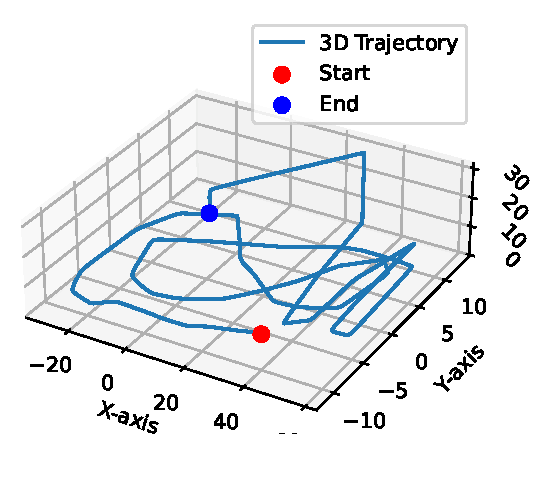
\includegraphics[width=\textwidth]{tex/ch5_airio/figs/pegasus_trajs/pegasus_3_train_test_sorted.pdf}
        \caption{TRAIN\_4: Distance 452.1$\si{\meter}$, Duration 160.4~\unit{\second}, Peak 4.9, Avg. 2.8~\unit{\metre\per\second}.}
        \label{fig:airio:sub_train4}
    \end{subfigure}
    \caption{Training trajectories (1--4).}
    \label{fig:airio:trainmain}
\end{figure}
